\documentclass[11pt]{article}
\usepackage[margin=1in]{geometry}
\usepackage{booktabs,graphicx,amsmath,amssymb,hyperref,xcolor,microtype,natbib,listings,enumitem}
\hypersetup{colorlinks=true,linkcolor=teal,citecolor=teal,urlcolor=teal}
\bibliographystyle{plainnat}
\definecolor{codebg}{RGB}{238,242,242}
\lstset{basicstyle=\ttfamily\footnotesize,backgroundcolor=\color{codebg},frame=none,breaklines=true,columns=fullflexible,
  keepspaces=true,showstringspaces=false,xleftmargin=4pt,xrightmargin=4pt,aboveskip=6pt,belowskip=6pt}
\newcommand{\step}[1]{\subsection*{#1}}
\newcommand{\SpeedupGemma}{10}
\newcommand{\FTMinutes}{85}
\newcommand{\AbstractResults}{Zero-shot, Kev-4B is the strongest decision model (lung AUROC 0.88, AAA 1.00, TREC 0.82--0.84, on par with an 8B generative LLM on TREC), while Laya is near chance, as its authors warn. Two steps account for most of the gain. An 85-minute on-laptop RLCD fine-tune of the 421M Laya encoder on synthetic notes lifts lung AUROC on 40 hand-written notes from 0.55 to 0.90 (0.999 on held-out templates). The arithmetic hook then raises the share of hand-written notes that can be auto-decided at $\leq$5\% error from 38\% to 85\% (AUROC 0.96), at 124\,ms per note, about 10$\times$ faster than the generative baseline, which reaches AUROC 0.99 with the same hook. Thresholds measured on template notes do not transfer to hand-written ones, which is why Step~5 must use the practitioner's own notes.}


\title{Checklists at the Speed of Prefill:\\[4pt]\large Local, Calibrated Clinical Eligibility Screening with Open Decision Models}
\author{Prahlad G. Menon\\\small The Menon Lab, University of Pittsburgh \quad \href{https://themenonlab.blog}{themenonlab.blog}}
\date{November 2026 (revised; first version September 2026)}

\begin{document}
\maketitle

\begin{abstract}
\noindent\textbf{Objective.}
Much of standard-of-care qualification means applying a published checklist to a free-text chart.
We asked whether open \emph{decision models}, a new class of models that answer typed yes/no questions with calibrated probabilities from a single prefill pass, can do this on a single laptop. We also asked which practical steps make them safe to use.

\noindent\textbf{Methods.}
We encoded the USPSTF 2021 lung-cancer and 2019 abdominal aortic aneurysm screening recommendations as one question per criterion, and combined the answers into an auditable conjunctive eligibility score.
We evaluated ten local systems on 900 synthetic notes from held-out templates with exact per-criterion labels, 40 hand-written notes, and 600 eligible-versus-excluded patient--trial pairs from TREC Clinical Trials 2021. Nine were decision models from four model families released between September and November 2026, and one was a generative large language model.
We tested a deterministic hook that states smoking arithmetic, an 85-minute on-laptop fine-tune from synthetic notes, and automation thresholds chosen for a fixed error budget.

\noindent\textbf{Results.}
\AbstractResults{}

\noindent\textbf{Conclusions.}
Open decision models can screen checklists locally, with no note leaving the machine, provided that the arithmetic is made explicit, the model is specialised or chosen on the target task, and the automation threshold is measured on the practitioner's own notes.
We release the pipeline as a step-by-step guide (Appendix~\ref{app:guide}), together with a local screening app, data generators and every prediction.
\end{abstract}

% =====================================================================
\section{Introduction}
\label{sec:intro}
Clinical qualification work often reduces to a checklist over a chart.
Examples are the USPSTF recommendation that adults aged 50--80 with a 20 pack-year smoking history be offered annual low-dose CT \citep{krist2021lung}, or a trial's inclusion and exclusion criteria.
The facts these checklists need often exist only in narrative text, such as ``1 ppd since he was 18'' or ``quit after his MI in 2019''.
Rule engines over structured fields miss them.
Generative large language models (LLMs) can read them \citep{jin2024trialgpt,wornow2024zeroshot}, but they are hard to run on premises.
Their free-text output must be parsed, and their confidence is not calibrated by default.

A new class of models answers \emph{typed questions} about a text in a single prefill pass: \emph{decision models}, also called System One models.
TypeSafe introduced the category on 15 September 2026 with Jev and its \texttt{/v1/systemone} API \citep{typesafe2026,typesafe_jev_docs}.
Within seven weeks it had become crowded:
\begin{itemize}[nosep]
\item OpenAI's Decisions API reached general availability \citep{openai_decisions}.
\item Microsoft, Liquid AI and others launched hosted models \citep{ms_decision1,liquid_d1}.
\item Perplexity, Cloudflare, H2O.ai, IBM and the vLLM project released open weights \citep{pplx_decider_v12,cloudflare_clef,h2o_lightning4b,granite_switch,vllmsr_decision2}.
\item Chrome prototyped an in-browser Decisions API \citep{chrome_decisions}, and llama.cpp added a native server for the API \citep{llamacpp_systemone}.
\item Independent leaderboards appeared \citep{decision_index,jevbench,aa_decision_index}, together with a first wave of clinical evaluations (\S\ref{sec:related}).
\end{itemize}
For a checklist the interface has the right shape: one question per criterion, one probability for each, and a principled basis for deciding which cases are safe to automate.

The field now offers dozens of models but no answer to the question a clinical team actually faces: \emph{how do we run our own checklist safely, on our own hardware, without sending notes anywhere?}
This paper addresses that question. Our contributions are:
\begin{enumerate}[nosep]
\item a screening pipeline that turns any public checklist into per-criterion decision questions with an auditable conjunctive score, written up as a step-by-step practitioner guide (Appendix~\ref{app:guide});
\item a controlled benchmark with exact per-criterion labels, held-out templates and hand-written notes, on which ten local systems are compared;
\item evidence that two inexpensive steps, a deterministic arithmetic hook and a short on-laptop fine-tune from synthetic notes, change which models are usable;
\item a measured demonstration that automation thresholds do not transfer from synthetic to hand-written notes;
\item an open-source release, including a local screening app, in which no note leaves the machine.
\end{enumerate}

% =====================================================================
\section{Background and related work}
\label{sec:related}

\subsection{Decision models}
A decision model reads a \emph{state} (a note, a JSON record) and a set of questions whose answers are declared up front, and returns a probability for every answer instead of generated text.
The System One API defines three question types: \texttt{noul} (yes/no), \texttt{choice} and \texttt{score} \citep{typesafe2026}.
The two open designs we study first span the range of architectures.
\textbf{Laya} \citep{laya2026} packs a question, its options (each introduced by a \texttt{[MASK]} marker) and the state into one sequence for a bidirectional encoder (ModernBERT-large, 421M parameters; \citealp{warner2024modernbert}), and a two-layer head scores each marker.
It is trained (``RLCD'') with a GRPO-style policy gradient \citep{shao2024grpo} on strictly proper scoring rules \citep{gneiting2007scoring} plus soft cross-entropy, and is then temperature-scaled \citep{guo2017calibration}.
\textbf{Kev} \citep{kev2026} freezes a Qwen3.5 base and trains a rank-16 LoRA \citep{hu2022lora} and a pointer head, which scores each option's closing token against a final \texttt{<decide>} token. The note is prefilled once, and each question reuses the cache.
Most open entrants since then (Table~\ref{tab:landscape}) follow Kev's pattern: a 4B--31B Qwen or Gemma decoder with a readout head, one temperature, and the System One request shape.
Because they share that request shape, one client can drive almost all of them.

\begin{table}[t]\centering\scriptsize
\caption{The decision-model landscape on 4 November 2026 (selection). ``S1'' = TypeSafe's \texttt{/v1/systemone} request shape. ``Mac'' = runs on a 64\,GB Apple-silicon laptop. DI = independent Decision Index 0.4.1 Full score \citep{decision_index} (chance-corrected, higher is better; ``--'' = not listed). Data-governance column quotes only what the provider states publicly; ``none stated'' means we found no statement, not that none exists. $^\dagger$ = evaluated in this paper.}
\label{tab:landscape}
\resizebox{\linewidth}{!}{\begin{tabular}{llllllr}\toprule
Model & Organisation (date) & Weights & Size / base & Interface & Clinical data governance (stated) & DI \\ \midrule
Jev 1.13 / 1.14 & TypeSafe (15 Sep / 14 Oct) & hosted & undisclosed & S1 (origin) & ZDR for enterprise; no HIPAA/BAA found & 60.2 \\
Decisions API (gpt-6-luna) & OpenAI (GA 22 Oct) & hosted & undisclosed & own (\texttt{/v1/decisions}) & ZDR and HIPAA for eligible customers & -- \\
Microsoft-Decision-1 & Microsoft (9 Oct) & hosted & Qwen3.5-9B & S1 & data zones; HIPAA not stated & -- \\
d1 / d1-ultra & Liquid AI (29 Sep) & hosted & undisclosed & S1 & none stated & -- \\
pplx-decider v1.2 (27B) & Perplexity (1--15 Oct) & open, Apache-2.0 & Qwen3.8-27B & S1-style & ZDR by agreement (hosted) & 68.0 \\
Clef / Clef-flash & Cloudflare (1 Oct) & open, Apache-2.0 & 27B / 9B (Qwen) & S1 & Workers AI: zero retention & 54.9 / 44.4 \\
H2O-Lightning-4B & H2O.ai (2 Oct) & open, Apache-2.0 & Qwen3.5-4B & S1 (llama.cpp) & local & -- \\
Decision 2.0 (Nox-4B \ldots{} Vega-27B) & vLLM Semantic Router (28 Sep) & open, Apache-2.0 & Qwen3.5/3.8 & S1 (llama.cpp) & local & -- \\
Granite Switch 4.1 & IBM (14 Oct) & open, Apache-2.0 & 8B / 30B & chat + S1 & local & -- \\
Decisions API (\texttt{DecisionModel}) & Google Chrome (prototype, Oct) & on-device & undisclosed & own web API & ``inputs not sent over the network'' & -- \\
Kev 1.0 (0.8B--27B) & J.\ Palmer (Sep--Oct) & open, Apache-2.0 & Qwen3.5/3.8 + LoRA & S1 & local & 59.6 (27B), 40.9 (9B), 34.9 (4B) \\
Laya & ConvAI Innovations (18 Sep) & open, Apache-2.0 & ModernBERT 421M & S1 & local & 9.2 \\
\midrule
MedJev & Lee et al.\ (26 Oct) & open, CC-BY-NC & 9B & S1 (shim) & local & -- \\
CS1-4B & Zhang et al.\ / Mahmood lab (19 Oct) & not released & Decision 2.0 Nox-4B & S1 & trained on 3.6M patients & -- \\
\bottomrule\end{tabular}}
\end{table}


\subsection{Independent benchmarks}
On the Hugging Face Decision Index \citep{decision_index}, the best open models (71--72) now score above Jev 1.14 (60.2).
Kev-27B (59.6) is level with Jev; Kev-4B scores 34.9, and Laya scores 9.2 and ranks 251st of 265.
JevBench \citep{jevbench} and the Artificial Analysis Decision Index \citep{aa_decision_index} give the same broad ordering, and find that decision models remain overconfident on knowledge questions.
These boards measure general-purpose decisions, not clinical checklists.
Laya's author has publicly claimed priority over Jev's architecture \citep{tomshw_dispute}; we cite both and take no position.

\subsection{Clinical eligibility from text}
Cohort selection from narrative records was benchmarked in the n2c2 2018 shared task \citep{stubbs2019n2c2}.
Criteria2Query translates free-text criteria into database queries \citep{yuan2019criteria2query}, and the TREC Clinical Trials track provides graded patient--trial judgements \citep{roberts2021trec}.
LLM-based matchers achieve strong criterion-level performance with large generative models, usually hosted \citep{jin2024trialgpt,wornow2024zeroshot}.

\subsection{Clinical evaluations of decision models}
Most early studies tested hosted Jev or large open decision models on medical knowledge and diagnosis.
Accuracy is reasonable on examination-style questions, but calibration degrades on patient-level prediction and complex cases \citep{du2026reliable,madrid2026rheum,you2026triage,deobhakta2026ddx}. Laya was ``near chance'' in rheumatology \citep{madrid2026rheum}.
Three studies are closest to ours:
\begin{itemize}[nosep]
\item \citet{he2026trial} evaluated hosted Jev under zero data retention on 2{,}048 TrialGPT and MIMIC patient--criterion pairs. It matched a schema-constrained LLM on macro-F1, flagged insufficient information more reliably, and cost 53--74\% less.
\item \citet{zhang2026cs1} trained CS1-4B from Decision 2.0 Nox-4B on 12.4M questions from 3.6M patients. It outperformed open models of up to 27B on 13 of 14 tasks and quadrupled the number of eligible patients in the top 20 for trial screening. Its weights are not public.
\item \citet{lee2026medjev} released MedJev and reported a patient-level ECE of 0.286, reduced to 0.007 by recalibration on 50--200 labelled examples.
\end{itemize}
These works evaluate models. We provide a procedure a practitioner can follow, which needs neither hospital-scale training data nor a data-processing agreement, and we test each of its steps.

\subsection{Selective prediction}
A calibrated probability allows a system to abstain.
We use the risk--coverage framework \citep{geifman2017selective}: cases are ranked by confidence, and we report the largest share that can be auto-decided while the error rate among them stays within a budget.

% =====================================================================
\section{Methods}
\label{sec:methods}

\subsection{Screening pipeline}
\label{sec:pipeline}
The pipeline has seven steps (full guide with code in Appendix~\ref{app:guide}):
\begin{enumerate}[nosep]
\item encode each criterion as a \texttt{noul} question with the answer that eligibility requires;
\item choose a local decision model and serve it behind the System One API;
\item optionally append deterministic arithmetic facts to the note;
\item combine the criterion probabilities into a conjunctive eligibility score;
\item choose an automation threshold on labelled notes for a fixed error budget;
\item if coverage is too low, fine-tune locally on synthetic notes;
\item deploy with clinician review of the cases below the threshold.
\end{enumerate}
The sections below specify each component as used in the experiments.

\subsection{Checklist encoding and the conjunctive score}
\label{sec:encoding}
The \textbf{lung-cancer screening} recommendation (USPSTF 2021, Grade B; \citealp{krist2021lung}) yields four criteria: age 50--80; $\geq$20 pack-years; currently smokes or quit $\leq$15 years ago; and no health problem that substantially limits life expectancy or the ability or willingness to undergo curative lung surgery. The last criterion must be answered ``no''.
The \textbf{AAA screening} recommendation (USPSTF 2019, Grade B; \citealp{owens2019aaa}) yields three: male, age 65--75, ever smoked.
Each criterion is a \texttt{noul} question stating its thresholds, inclusivity and units (Appendix~\ref{app:questions}).
For criteria $c_i$ with required answers $r_i\in\{\text{yes},\text{no}\}$ and model probabilities $p_i=P(c_i=\text{yes}\mid\text{note})$, the conjunctive score is
\begin{equation}
P(\text{eligible}) = \textstyle\prod_i \big[p_i\,\mathbf{1}(r_i=\text{yes}) + (1-p_i)\,\mathbf{1}(r_i=\text{no})\big].
\label{eq:and}
\end{equation}
This treats the criteria as conditionally independent given the note, which is a heuristic. In return, every negative decision names the criterion responsible.
As a comparison we also ask a single \emph{direct} question containing the whole recommendation.

\subsection{Computed-facts hook}
\label{sec:facts}
Decision models are weakest where a checklist needs arithmetic: packs per day $\times$ years, cigarettes converted to packs, or a quit year compared with the visit year.
A deterministic pre-processor (\texttt{clinical\_system1/facts.py}) finds these spans with generic regular expressions and appends the computed values, for example \texttt{[Computed facts: about 40 pack-years (1 packs/day x 40 years); age 58.]}.
The model still makes every judgement. When no pattern matches, nothing is appended.
This mirrors Kev's \texttt{KEV\_DATE\_FACTS} option for day counts.

\subsection{Data}
\label{sec:data}
\paragraph{E1: synthetic vignettes.}
Primary-care notes are rendered from structured seeds (age, sex, smoking status, packs per day, years smoked, years since quitting, life-limiting condition, refusal of surgery), so every criterion label is exact.
Smoking history is phrased as packs/day $\times$ years, cigarettes/day $\times$ years, or a stated pack-year figure; quitting is phrased as ``$N$ years ago'' or ``in YYYY'' with the visit year given.
Distractors include household smoking, secondhand exposure, a family history of lung cancer or AAA, and benign comorbidities.
Life-limiting conditions are:
\begin{itemize}[nosep]
\item hospice-enrolled metastatic cancer;
\item NYHA~IV heart failure;
\item oxygen-dependent end-stage COPD;
\item advanced dementia;
\item ESRD with dialysis declined;
\item explicit refusal of surgery.
\end{itemize}
Values at each threshold are oversampled.
Template family A (bullet and short narrative formats; 3{,}000 lung and 2{,}000 AAA notes) is used only for fine-tuning and calibration.
Family B (problem-list and long-narrative formats; 500 lung and 400 AAA notes, 40\% eligible) is used only for testing.
\paragraph{E1b: hand-written notes.}
We wrote 40 free-text notes by hand with clinical abbreviations (``ppd'', ``pk-yr'', ``s/p''), indirect dates (``quit after his MI in 2019'') and boundary cases (e.g.\ 10 cigarettes/day for 38 years = 19 pack-years). 13 are lung-eligible and 10 AAA-eligible.
\paragraph{E2: trial prescreening.}
From TREC Clinical Trials 2021 \citep{roberts2021trec} we sampled 600 judged patient--trial pairs, 300 eligible and 300 excluded, stratified over the 75 topics.
Eligibility text was taken from the ClinicalTrials.gov v2 API, with each criteria block capped at 6{,}000 characters.
We ask a direct eligibility question plus ``meets the inclusion criteria?'' and ``meets any exclusion criterion?'', and score $P(\text{inc})(1-P(\text{exc}))$.

\subsection{Models}
\label{sec:systems}
All systems run locally on one Apple M1 Max laptop (64\,GB unified memory). Table~\ref{tab:systems} lists them.
Kev-0.8B, Kev-4B and Kev-9B are served by Kev's own MLX server; Kev-27B, H2O-Lightning-4B and Clef-flash by llama.cpp's native \texttt{/v1/systemone} endpoint (build 11960). Two settings were needed on this hardware: \nolinkurl{GGML_METAL_BF16_DISABLE=1}, because the M1 GPU lacks bfloat16, and, for Clef-flash, a physical batch at least as long as the input (\nolinkurl{-b 16384 -ub 16384}).
All decision models are queried through the same System One client with their shipped calibration.
We do not apply H2O's optional ``yes/no floor'', which changes reported probabilities.
The generative baseline, Gemma~4 (about 8B, 4-bit, via Ollama), is asked one question at a time; $P(\text{yes})$ is the softmax over its first-token log-probabilities for ``Yes'' and ``No''.
For time reasons Gemma~4 was run on the first 250 notes of each E1 template test set and a balanced 300-pair E2 subset. Kev-27B (about 5\,s per note) was run on the first 250 notes of each E1 template test set, all hand-written notes, and a balanced 150-pair E2 subset.
We tried to include further medical and open models but excluded them for reproducibility reasons:
\begin{itemize}[nosep]
\item MedJev \citep{medjev_weights} and MedDecider (non-commercial) require bespoke client runtimes from their model repositories;
\item a community GGUF of pplx-decider was incompatible with stock llama.cpp;
\item Decision 2.0 Nox-4B, the base of CS1-4B, needs a llama.cpp build newer than the packaged release.
\end{itemize}

\begin{table}[t]\centering\small
\caption{Systems evaluated. All run on one Apple M1 Max (64\,GB). FT = fine-tuned in this work.}
\label{tab:systems}
\begin{tabular}{llll}\toprule
System & Parameters / precision & Runtime & Released \\ \midrule
Laya EN, Laya multilingual (zero-shot) & 421M / 322M, fp32 & PyTorch MPS & Sep 2026 \\
Laya EN + RLCD FT (ours) & 421M, fp32 & PyTorch MPS & this work \\
Kev-0.8B, Kev-4B, Kev-9B v2 & LoRA on Qwen3.5, bf16 & Kev MLX server & Sep--Oct 2026 \\
Kev-27B v2 & 27B, Q4\_K\_M GGUF & llama.cpp & Oct 2026 \\
H2O-Lightning-4B & 4B, Q8\_0 GGUF & llama.cpp & Oct 2026 \\
Cloudflare Clef-flash & 9B, Q8\_0 GGUF & llama.cpp & Oct 2026 \\
Gemma~4 (generative reference) & $\sim$8B, 4-bit & Ollama & 2026 \\
\bottomrule\end{tabular}
\end{table}

\subsection{Local fine-tuning}
\label{sec:ft}
We ported Laya's released two-GPU RLCD notebook to a single Apple GPU, keeping its hyperparameters:
\begin{itemize}[nosep]
\item AdamW with learning rates $2.5\times10^{-5}$ (encoder) and $10^{-4}$ (head), cosine schedule;
\item micro-batch 8 with 4-step accumulation;
\item $G{=}4$ noisy samples, with $\sigma$ annealed from 0.4 to 0.1;
\item a reward combining log, spherical ($w{=}0.75$) and ranked-probability ($w{=}1$) scores, plus soft cross-entropy.
\end{itemize}
Laya's maintainers have since published their own Apple-silicon script. We trained for 2 epochs on 22{,}000 criterion and direct questions from family A, then fitted a \texttt{noul} temperature by LBFGS on 1{,}000 held-out family-A questions.
Family-B notes and hand-written notes were never seen in training or calibration.

\subsection{Automation thresholds and metrics}
\label{sec:metrics}
For a score $P$, confidence is $\max(P,1-P)$ and the decision is $P\geq0.5$.
Notes are ranked by confidence. \emph{Coverage at budget $b$} is the largest fraction of notes that can be auto-decided, most confident first, with an error rate $\leq b$ among them; the corresponding confidence is the automation threshold $\tau$.
We also report AUROC with 95\% bootstrap confidence intervals (1{,}000 resamples), accuracy at 0.5, balanced accuracy, Brier score, 10-bin expected calibration error (ECE), and the fraction of notes on which every criterion is answered correctly (``all criteria right'').
Latency is the median wall-clock time per note for the full five-question lung checklist, measured with nothing else running on the GPU.

% =====================================================================
\section{Results}
\label{sec:results}

\begin{figure}[t]\centering
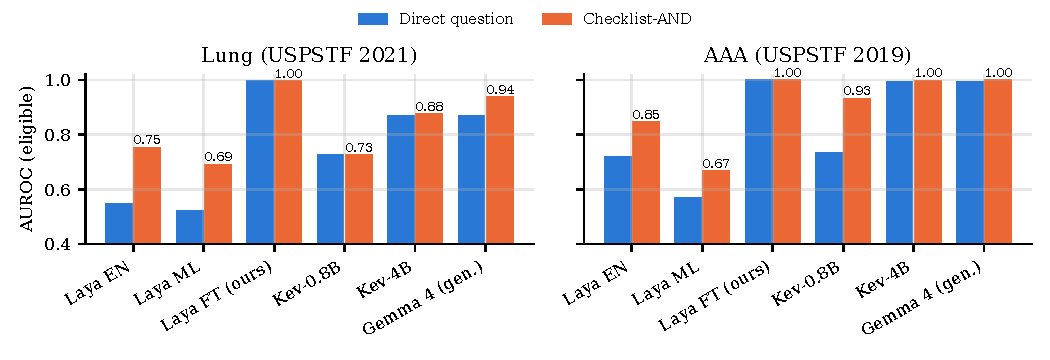
\includegraphics[width=\linewidth]{figures/auroc_e1.pdf}
\caption{Eligibility AUROC on held-out-template notes: one direct question (blue) versus the conjunctive score (orange).}
\label{fig:auroc}
\end{figure}
\begin{table}[t]\centering\small
\caption{USPSTF 2021 lung cancer screening eligibility on 500 held-out-template notes (40\% eligible). Coverage = share of notes auto-decided at the given error budget. Bold = best.}\label{tab:lcs}
\resizebox{\linewidth}{!}{\begin{tabular}{lrrrrrrrr}\toprule
 & Direct & \multicolumn{5}{c}{Checklist-AND} & All crit. & \\ \cmidrule(lr){2-2}\cmidrule(lr){3-7}
Model & AUROC & AUROC & Acc & Brier$\downarrow$ & Cov@5\% & Cov@10\% & correct & $n$ \\ \midrule
Laya EN (0-shot) & 0.547 & 0.754 & 0.600 & 0.369 & 0.130 & 0.168 & 0.082 & 500 \\
Laya ML (0-shot) & 0.523 & 0.693 & 0.608 & 0.284 & 0.000 & 0.130 & 0.242 & 500 \\
Laya EN + RLCD FT (ours) & \textbf{0.998} & \textbf{0.999} & \textbf{0.992} & \textbf{0.008} & \textbf{1.000} & \textbf{1.000} & \textbf{0.972} & 500 \\
Kev-0.8B & 0.726 & 0.728 & 0.602 & 0.260 & 0.268 & 0.316 & 0.288 & 500 \\
Kev-4B & 0.872 & 0.877 & 0.648 & 0.244 & 0.424 & 0.492 & 0.402 & 500 \\
Kev-9B v2 & 0.903 & 0.890 & 0.602 & 0.289 & 0.390 & 0.466 & 0.166 & 500 \\
H2O-Lightning-4B & 0.929 & 0.919 & 0.632 & 0.219 & 0.370 & 0.568 & 0.508 & 500 \\
Gemma~4 (generative) & 0.870 & 0.940 & 0.888 & 0.085 & 0.776 & 0.924 & 0.712 & 250 \\
\bottomrule\end{tabular}}\end{table}
\begin{table}[t]\centering\small
\caption{Lung screening on 40 hand-written free-text notes (13 eligible).}\label{tab:lcshand}
\resizebox{\linewidth}{!}{\begin{tabular}{lrrrrrrrr}\toprule
 & Direct & \multicolumn{5}{c}{Checklist-AND} & All crit. & \\ \cmidrule(lr){2-2}\cmidrule(lr){3-7}
Model & AUROC & AUROC & Acc & Brier$\downarrow$ & Cov@5\% & Cov@10\% & correct & $n$ \\ \midrule
Laya EN (0-shot) & 0.462 & 0.553 & 0.675 & 0.302 & 0.075 & 0.075 & 0.100 & 40 \\
Laya ML (0-shot) & 0.590 & 0.293 & 0.675 & 0.302 & 0.025 & 0.025 & 0.175 & 40 \\
Laya EN + RLCD FT (ours) & \textbf{0.913} & \textbf{0.903} & \textbf{0.875} & \textbf{0.122} & 0.375 & \textbf{0.750} & \textbf{0.850} & 40 \\
Kev-0.8B & 0.821 & 0.553 & 0.675 & 0.238 & 0.100 & 0.100 & 0.375 & 40 \\
Kev-4B & 0.869 & 0.732 & 0.650 & 0.254 & 0.275 & 0.325 & 0.500 & 40 \\
Kev-9B v2 & 0.880 & 0.752 & 0.675 & 0.259 & 0.250 & 0.425 & 0.225 & 40 \\
H2O-Lightning-4B & 0.846 & 0.832 & 0.675 & 0.205 & 0.550 & 0.575 & 0.575 & 40 \\
Cloudflare Clef-flash 9B & 0.889 & 0.883 & 0.700 & 0.166 & 0.550 & 0.600 & 0.700 & 40 \\
Kev-27B v2 (Q4) & 0.895 & 0.897 & 0.775 & 0.152 & \textbf{0.575} & 0.625 & 0.725 & 40 \\
Gemma~4 (generative) & 0.838 & 0.840 & 0.800 & 0.163 & 0.250 & 0.600 & 0.650 & 40 \\
\bottomrule\end{tabular}}\end{table}

\subsection{Zero-shot performance of decision models}
\label{sec:res-zeroshot}
Tables~\ref{tab:lcs}--\ref{tab:aaa} and Figure~\ref{fig:auroc} summarise the checklist results.
\textbf{The newer open decision models are markedly stronger zero-shot.}
On the lung template notes the conjunctive AUROC is 0.976 for Clef-flash (9B) and 0.919 for H2O-Lightning-4B, against 0.877 for Kev-4B and 0.890 for Kev-9B.
The gap is clearest in the audit trail: every criterion is right on 80\% of notes for Clef-flash, 51\% for H2O-Lightning-4B, and 40\% and 17\% for Kev-4B and Kev-9B. Kev-9B mislabels the life-limiting criterion on most notes.
Kev-27B (250 notes, 4-bit) reaches a conjunctive AUROC of 0.977 with every criterion right on 73\% of notes.
AAA, whose criteria are stated explicitly, is essentially solved by every Kev model from 4B upward and by both new models (AUROC $\geq$0.998).
\textbf{Laya zero-shot is not usable} for this task. Lung AUROC is 0.55--0.75, all four criteria are right on only 8\% of notes, and it misjudges even the explicit age criterion (44\% accuracy). This matches its position near the bottom of the general leaderboards and upstream's warning that the \texttt{noul} head can follow its label text instead of the state.

\subsection{Which criteria fail}
\label{sec:res-criteria}
Arithmetic criteria are the bottleneck for every zero-shot model (Table~\ref{tab:crit}).
For Kev-4B, age is 98\% correct but pack-years only 77\% and recency 68\%; Kev-9B is similar on recency (69\%).
The newer models handle arithmetic better but not perfectly: pack-years 88\% and 91\%, and recency 80\% and 91\%, for H2O-Lightning-4B and Clef-flash respectively.
Kev-27B scores 88\% on pack-years and 92\% on recency.
\begin{table}[t]\centering\small
\caption{Per-criterion accuracy on the lung-screening test set (500 notes, template family B).}\label{tab:crit}
\begin{tabular}{lrrrr}\toprule Model & Age 50--80 & $\geq$20 pack-yr & Recency & Limiting \\ \midrule
Laya EN (0-shot) & 0.444 & 0.592 & 0.486 & 0.562 \\
Laya ML (0-shot) & 0.708 & 0.634 & 0.520 & 0.878 \\
Laya EN + RLCD FT (ours) & 1.000 & 0.992 & 0.980 & 1.000 \\
Kev-0.8B & 0.722 & 0.686 & 0.622 & 0.922 \\
Kev-4B & 0.982 & 0.774 & 0.682 & 0.830 \\
Kev-9B v2 & 0.934 & 0.886 & 0.686 & 0.298 \\
H2O-Lightning-4B & 0.940 & 0.876 & 0.804 & 0.774 \\
Gemma~4 (generative) & 0.968 & 0.840 & 0.888 & 0.976 \\
\bottomrule\end{tabular}\end{table}

\subsection{Effect of the computed-facts hook}
\label{sec:res-facts}
The hook raises pack-year accuracy for every model (Table~\ref{tab:facts}). Kev-4B goes from 0.77 to 0.98 on template notes and from 0.82 to 1.00 on hand-written notes; Gemma~4 goes from 0.84 to 0.99.
For the fine-tuned Laya on hand-written notes, AUROC rises from 0.903 to 0.957 and coverage at a 5\% error budget from 38\% to 85\%.
Kev's \emph{recency} accuracy does not change (0.68) even when ``quit about 16 years before the visit'' is stated, which indicates that it does not reliably compare a stated number with the 15-year cut-off inside a disjunctive question.
The newer models benefit as much. With the hook, Clef-flash reaches pack-year and recency accuracies of 1.00 and 0.97 on hand-written notes, and AUROC 1.000 (direct) and 0.997 (conjunctive). H2O-Lightning-4B reaches 1.00 and 1.00, with AUROC 0.989 (direct). Kev-27B reaches AUROC 1.000 (direct) and 0.997 (conjunctive), and the highest safe-automation share in the study on hand-written notes (95\% at a 5\% error budget with the conjunctive score; 100\% with the direct question).
The hook can also hurt. For H2O-Lightning-4B on template notes, accuracy on the unrelated life-limiting criterion fell from 0.77 to 0.59 when facts were appended, so any hook must be validated on every criterion, not just the ones it targets.
The hook computed pack-years for all 433 template smokers and for 34 of the 36 hand-written smokers. The two misses were ``from her 20s until 2005'' and ``a few cigarettes on weekends''.
\begin{table}[t]\centering\small
\caption{Step 3 ablation: the computed-facts hook on the lung checklist (checklist-AND). $\Delta$ = with minus without.}\label{tab:facts}
\resizebox{\linewidth}{!}{\begin{tabular}{llrrrrr}\toprule Notes & Model & AUROC & Pack-yr acc & Recency acc & Cov@5\% & All crit. \\ \midrule
Template & Kev-0.8B & 0.81 (+0.08) & 0.84 (+0.16) & 0.63 (+0.01) & 0.35 (+0.08) & 0.34 (+0.06) \\
Template & Kev-4B & 0.94 (+0.06) & 0.98 (+0.20) & 0.68 (+0.00) & 0.52 (+0.10) & 0.44 (+0.04) \\
Template & Kev-9B v2 & 0.97 (+0.08) & 1.00 (+0.11) & 0.68 (-0.00) & 0.55 (+0.16) & 0.19 (+0.03) \\
Template & H2O-Lightning-4B & 0.96 (+0.05) & 0.99 (+0.12) & 0.92 (+0.11) & 0.42 (+0.05) & 0.52 (+0.01) \\
Template & Cloudflare Clef-flash 9B & 1.00 (+0.02) & 1.00 (+0.09) & 0.98 (+0.07) & 0.96 (+0.30) & 0.92 (+0.12) \\
Template & Kev-27B v2 (Q4) & 1.00 (+0.02) & 1.00 (+0.12) & 0.98 (+0.06) & 1.00 (+0.08) & 0.88 (+0.15) \\
Template & Laya EN (0-shot) & 0.70 (-0.06) & 0.75 (+0.16) & 0.70 (+0.21) & 0.18 (+0.05) & 0.11 (+0.03) \\
Template & Laya EN + RLCD FT (ours) & 0.99 (-0.00) & 1.00 (+0.01) & 0.94 (-0.04) & 1.00 (+0.00) & 0.93 (-0.04) \\
Template & Gemma~4 (generative) & 1.00 (+0.06) & 0.99 (+0.15) & 0.92 (+0.03) & 1.00 (+0.22) & 0.88 (+0.16) \\
\midrule
Hand-written & Kev-0.8B & 0.64 (+0.09) & 0.85 (+0.05) & 0.70 (-0.03) & 0.15 (+0.05) & 0.42 (+0.05) \\
Hand-written & Kev-4B & 0.76 (+0.03) & 1.00 (+0.18) & 0.68 (+0.00) & 0.25 (-0.03) & 0.55 (+0.05) \\
Hand-written & Kev-9B v2 & 0.87 (+0.11) & 1.00 (+0.12) & 0.68 (+0.00) & 0.50 (+0.25) & 0.25 (+0.02) \\
Hand-written & H2O-Lightning-4B & 0.95 (+0.12) & 1.00 (+0.20) & 1.00 (+0.18) & 0.65 (+0.10) & 0.72 (+0.15) \\
Hand-written & Cloudflare Clef-flash 9B & 1.00 (+0.11) & 1.00 (+0.18) & 0.97 (+0.07) & 0.82 (+0.27) & 0.90 (+0.20) \\
Hand-written & Kev-27B v2 (Q4) & 1.00 (+0.10) & 1.00 (+0.10) & 0.97 (+0.15) & 0.95 (+0.38) & 0.90 (+0.18) \\
Hand-written & Laya EN (0-shot) & 0.76 (+0.21) & 0.78 (+0.22) & 0.62 (+0.10) & 0.40 (+0.33) & 0.20 (+0.10) \\
Hand-written & Laya EN + RLCD FT (ours) & 0.96 (+0.05) & 0.95 (+0.10) & 0.93 (-0.05) & 0.85 (+0.47) & 0.88 (+0.03) \\
Hand-written & Gemma~4 (generative) & 0.99 (+0.15) & 0.97 (+0.12) & 0.82 (+0.05) & 0.80 (+0.55) & 0.78 (+0.12) \\
\bottomrule\end{tabular}}\end{table}

\subsection{Direct question versus conjunctive score}
\label{sec:res-and}
On template notes the conjunctive score is at least as good as the direct question for every system (e.g.\ Gemma~4 lung 0.870$\rightarrow$0.940; Kev-0.8B AAA 0.736$\rightarrow$0.934), and its audit trail is fully correct on 97\% of notes for the fine-tuned Laya.
It is not uniformly better. For zero-shot Kev on hand-written lung notes the direct question wins (Kev-4B 0.869 vs 0.732; with facts 0.966 vs 0.764), because a single miscalibrated criterion (recency) pulls the product down and sensitivity falls to 0.15.
The same pattern, high AUROC but low sensitivity at a 0.5 cut-off, appears for most zero-shot models, because a product of four moderately confident ``yes'' answers rarely exceeds 0.5. This is a further reason to set the operating point on labelled notes rather than at 0.5.

\subsection{Local fine-tuning}
\label{sec:res-ft}
Fine-tuning took 85 minutes and fitted a \texttt{noul} temperature of 3.5 (0.996 accuracy on the held-out calibration slice).
On the unseen family-B templates the fine-tuned Laya reaches lung AUROC 0.999 and AAA 1.000, with Brier 0.008 and every criterion right on 97\% of notes.
Because the two template families share phrase vocabulary, the hand-written notes are the stricter test.
There it scores lung AUROC 0.903 (0.957 with facts), with every criterion right on 85\% (87.5\%) of notes, compared with 0.553 and 10\% before fine-tuning.
On hand-written notes the fine-tuned 421M encoder is therefore competitive with the strongest zero-shot models in the study (conjunctive AUROC without/with facts: Kev-27B 0.897/0.997; Clef-flash 0.883/0.997; H2O-Lightning-4B 0.832/0.949), at between a tenth and a fortieth of their latency, although the 27B model automates more notes safely (95\% vs 85\%). With only 40 notes the confidence intervals of the top systems overlap (Table~\ref{tab:lcshand}).
\begin{table}[t]\centering\small
\caption{USPSTF 2019 AAA screening eligibility on 400 held-out-template notes (40\% eligible).}\label{tab:aaa}
\resizebox{\linewidth}{!}{\begin{tabular}{lrrrrrrrr}\toprule
 & Direct & \multicolumn{5}{c}{Checklist-AND} & All crit. & \\ \cmidrule(lr){2-2}\cmidrule(lr){3-7}
Model & AUROC & AUROC & Acc & Brier$\downarrow$ & Cov@5\% & Cov@10\% & correct & $n$ \\ \midrule
Laya EN (0-shot) & 0.720 & 0.849 & 0.600 & 0.300 & 0.417 & 0.468 & 0.285 & 400 \\
Laya ML (0-shot) & 0.571 & 0.669 & 0.630 & 0.229 & 0.007 & 0.028 & 0.355 & 400 \\
Laya EN + RLCD FT (ours) & \textbf{1.000} & \textbf{1.000} & \textbf{1.000} & 0.000 & \textbf{1.000} & \textbf{1.000} & \textbf{1.000} & 400 \\
Kev-0.8B & 0.736 & 0.934 & 0.848 & 0.131 & 0.527 & 0.777 & 0.613 & 400 \\
Kev-4B & 0.993 & 1.000 & 0.988 & 0.017 & \textbf{1.000} & \textbf{1.000} & 0.965 & 400 \\
Kev-9B v2 & 0.998 & 0.998 & 0.983 & 0.018 & \textbf{1.000} & \textbf{1.000} & 0.965 & 400 \\
H2O-Lightning-4B & 1.000 & \textbf{1.000} & 0.988 & 0.026 & \textbf{1.000} & \textbf{1.000} & 0.990 & 400 \\
Gemma~4 (generative) & 0.994 & \textbf{1.000} & \textbf{1.000} & \textbf{0.000} & \textbf{1.000} & \textbf{1.000} & 0.996 & 250 \\
\bottomrule\end{tabular}}\end{table}

\subsection{Selective automation and threshold transfer}
\label{sec:res-threshold}
Coverage at a fixed error budget is the most practical quantity here and also the most fragile (Figure~\ref{fig:rc}).
The fine-tuned Laya automates 100\% of template notes at $\leq$5\% error with $\tau{=}0.98$, but only 38\% of hand-written notes (85\% with the facts hook).
Kev-4B automates 42\% of template notes but 28\% of hand-written ones. The stronger new models degrade less: Kev-27B with facts falls from 100\% to 95\% and Clef-flash with facts from 96\% to 82\% (conjunctive score), and H2O-Lightning-4B with facts and the direct question from 100\% to 90\%.
A threshold measured on synthetic notes would therefore overstate safe coverage on real text, by a factor of 2.6 for the fine-tuned model.
\begin{figure}[t]\centering
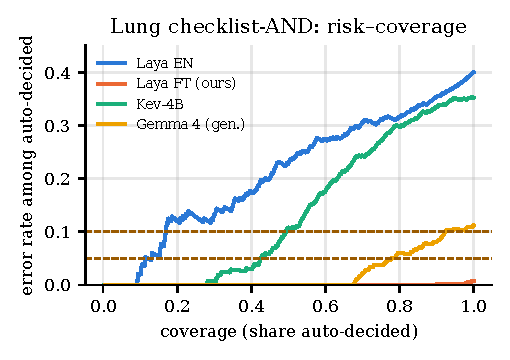
\includegraphics[width=.62\linewidth]{figures/risk_coverage.pdf}
\caption{Risk--coverage for the lung conjunctive score on held-out-template notes. A curve that stays under the dashed error budget longer automates more notes.}
\label{fig:rc}
\end{figure}

\subsection{Trial prescreening}
\label{sec:res-trec}
Distinguishing eligible from excluded patients for a topically relevant trial is harder (Table~\ref{tab:trec}).
Kev-4B reaches AUROC 0.820 [0.78, 0.85] directly and 0.839 [0.81, 0.87] with the inclusion$\times$(1$-$exclusion) decomposition. Kev-9B is similar (0.833 / 0.836) and Gemma~4 slightly lower (0.803 / 0.797).
The newer models are slightly better: H2O-Lightning-4B reaches 0.847 [0.82, 0.88] and Clef-flash 0.836 [0.80, 0.87]; Kev-27B reaches 0.903 [0.86, 0.94] on a balanced 150-pair subset.
The differences among the 4B--9B decision models are within their confidence intervals; all 4B--27B decision models score above the generative baseline (0.803).
Safe automation is limited: at a 5\% error budget the 4B--9B models auto-decide at most 13\% of pairs (best of the two scores), and the generative baseline 12\%. Kev-27B reaches 32\% with the direct question. In this setting trial prescreening is mainly a triage aid, with the largest model beginning to make partial automation plausible.
\begin{table}[t]\centering\small
\caption{TREC Clinical Trials 2021, eligible vs.\ excluded (balanced; 95\% bootstrap CI for AUROC).}\label{tab:trec}
\begin{tabular}{lrrrrr}\toprule & \multicolumn{2}{c}{Direct} & \multicolumn{2}{c}{Inc.$\times$(1$-$Exc.)} & \\ \cmidrule(lr){2-3}\cmidrule(lr){4-5}
Model & AUROC & Bal.\ acc & AUROC & Bal.\ acc & $n$ \\ \midrule
Laya ML (8k ctx) & 0.514 [0.47, 0.56] & 0.503 & 0.481 [0.43, 0.53] & 0.500 & 600 \\
Kev-0.8B & 0.633 [0.59, 0.68] & 0.515 & 0.627 [0.58, 0.67] & 0.587 & 600 \\
Kev-4B & 0.820 [0.78, 0.85] & 0.732 & 0.839 [0.81, 0.87] & 0.652 & 600 \\
Gemma~4 (generative) & 0.803 [0.75, 0.85] & 0.560 & 0.797 [0.74, 0.84] & 0.623 & 300 \\
\bottomrule\end{tabular}\end{table}

\subsection{Latency}
\label{sec:res-latency}
For the full five-question lung checklist on one M1 Max (Table~\ref{tab:lat}), the fine-tuned Laya takes 124\,ms per note on the GPU and 506\,ms on the CPU alone.
Kev-0.8B takes 134\,ms, Kev-4B 694\,ms and Gemma~4 1{,}250\,ms.
Through llama.cpp, H2O-Lightning-4B takes about 1.05\,s per note and Clef-flash about 1.47\,s; Kev-9B takes 1.58\,s and Kev-27B (4-bit) about 5.4\,s.
At 124\,ms per note, a single laptop screens about 29{,}000 notes per hour.
\begin{table}[t]\centering\small
\caption{Latency for the full 5-question lung checklist per note on one Apple M1 Max, uncontended (50 notes after 3 warm-up calls).}\label{tab:lat}
\begin{tabular}{llrrr}\toprule System & Params & p50 ms & p90 ms & notes/s \\ \midrule
Laya EN, Apple GPU (MPS) & 421M & 126 & 136 & 7.96 \\
Laya EN, CPU only & 421M & 506 & 571 & 1.93 \\
Laya FT (ours), MPS & 421M & 124 & 136 & 8.04 \\
Kev-0.8B, MLX bf16 & 0.8B & 134 & 137 & 7.68 \\
Kev-4B, MLX bf16 & 4B & 694 & 703 & 1.49 \\
Gemma~4, Ollama & $\sim$8B & 1250 & 1373 & 0.79 \\
Kev-9B v2, MLX bf16$^*$ & 9B & 1575 & 1730 & 0.64 \\
Kev-27B v2, llama.cpp Q4$^*$ & 27B & 5354 & 5841 & 0.19 \\
H2O-Lightning-4B, llama.cpp Q8$^*$ & 4B & 1053 & 1135 & 0.95 \\
Clef-flash, llama.cpp Q8$^*$ & 9B & 1468 & 1546 & 0.68 \\
\midrule\multicolumn{5}{l}{\footnotesize $^*$ median over all 500 lung test notes from the benchmark run itself (uncontended, sequential).}\\
\bottomrule\end{tabular}\end{table}

% =====================================================================
\section{Discussion}
\label{sec:discussion}

\subsection{Principal findings}
Five findings matter most for practice.
\begin{enumerate}[nosep]
\item The typed-question interface maps onto clinical checklists with no glue code and yields a per-criterion audit trail.
\item Open decision models improved sharply between September and November 2026. The strongest 4B--9B models released in October (H2O-Lightning-4B, Clef-flash) screen explicit criteria nearly perfectly zero-shot and are much better than earlier open models on criteria that need arithmetic.
\item Stating the arithmetic with a deterministic hook was the single most effective step for every model, and with it the best zero-shot open model reached AUROC 1.000 on hand-written lung notes. The hook can also degrade an unrelated criterion, so it must be validated on all of them.
\item A short on-laptop fine-tune turned the weakest model on the general leaderboards into one competitive with the strongest zero-shot models on this checklist, at a tenth to a fortieth of their latency, although the largest model still automated more notes safely. Specialisation from synthetic notes is a practical option when throughput or CPU-only deployment matters.
\item The automation threshold must be measured on the target notes. A threshold taken from synthetic data overstated safe coverage by up to 2.6-fold, less for stronger models (Kev-27B 100\% vs 95\%) but never zero.
\end{enumerate}

\subsection{Comparison with prior work}
Our threshold finding agrees with \citet{lee2026medjev}: out-of-the-box calibration of decision models on patient-level tasks is poor, and a small labelled set (50--200 examples) is enough to repair it.
CS1-4B \citep{zhang2026cs1} shows what institution-scale clinical training achieves. Our fine-tuning result suggests that much of the benefit for a fixed checklist is available from synthetic notes on a laptop, although our task is far narrower than theirs.
\citet{he2026trial} found hosted Jev competitive with a schema-constrained LLM on trial criteria; our TREC results show that open models running locally reach AUROC above 0.8 on a related task, although the two settings are not directly comparable.
General leaderboards were a partial guide. The models that rank highest among those we could run (Kev-27B, Clef-flash) were also strong here, but the model ranked 251st of 265 on the Decision Index became competitive after fine-tuning.

\subsection{Hosted or local deployment}
Hosted decision APIs are now inexpensive (\$0.01--0.10 per million input tokens), fast, and in some cases ahead on general leaderboards.
For clinical notes the deciding factor is usually governance.
Among the providers in Table~\ref{tab:landscape}, only OpenAI states HIPAA eligibility, and Cloudflare states zero data retention; the others offer retention terms under enterprise or written agreements, or make no statement.
A fully local pipeline needs no agreement, and the step that matters most, measuring the threshold on one's own notes, is the same in either deployment.

\subsection{Decision models and generative models}
In our September experiments the generative baseline was the most accurate system on hand-written lung notes. That is no longer the case.
With the facts hook, Gemma~4 reached AUROC 0.986 (conjunctive) and Clef-flash reached 0.997 (conjunctive) and 1.000 (direct), at similar latency on this laptop (1.25\,s and 1.47\,s per note).
The decision model returns calibrated probabilities through a standard API with no output parsing; the generative model needs one decode per question and a custom log-probability readout.
For high-throughput or CPU-only settings, the fine-tuned 421M encoder remains about ten times faster than either.

\subsection{Limitations}
\begin{itemize}[nosep]
\item \textbf{Synthetic text.} E1 notes are template-generated. Disjoint template families and hand-written notes narrow the gap to real EHR text but do not close it.
\item \textbf{Small hand-written set.} It contains 40 notes, written and labelled by the same author who wrote the facts hook, which may favour the hook.
\item \textbf{TREC data.} TREC topics are synthetic and its relevance labels are noisy.
\item \textbf{Independence assumption.} The conjunctive score treats criteria as independent given the note.
\item \textbf{Local models only.} We evaluated open models that run locally, several in quantised form; hosted APIs are discussed only from published information. The generative baseline is a single 4-bit model without chain-of-thought.
\item \textbf{Not validated for care.} Nothing here is validated for patient care. Deployment requires prospective evaluation on real charts, subgroup audits and clinician review of automated negatives.
\end{itemize}

% =====================================================================
\section{Conclusion}
Open decision models running on a laptop can screen standard-of-care checklists in a meaningful way, with no note leaving the machine.
This requires that the checklist be broken into typed criteria, the arithmetic be made explicit, the model be chosen or specialised on the target task, and the automation threshold be measured on the practitioner's own notes.
On our benchmark, the best zero-shot open model with an arithmetic hook reached AUROC 1.000 on hand-written lung notes, and a 421M encoder fine-tuned for 85 minutes on a laptop reached 0.957 at 124\,ms per note. In both cases the share of notes that could be automated safely had to be measured on the target notes.
The released guide, app and predictions allow others to repeat the process for their own checklists.

\section*{Data and code availability}
Code, vignette generators, hand-written notes, per-item predictions, the screening app and HTML documentation are available at \url{https://github.com/menonpg/clinical-system1} (Apache-2.0).
TREC Clinical Trials 2021 topics and judgements are available from NIST, and trial text from ClinicalTrials.gov.
Upstream models: \url{https://github.com/NandhaKishorM/laya}, \url{https://github.com/jaredpalmer/kev}, and the model cards cited in Table~\ref{tab:landscape}.

\section*{Use of AI assistance}
Software, experiment orchestration and manuscript drafting were assisted by an AI coding assistant (Claude, Anthropic). The author designed the study, reviewed all code and results, and takes responsibility for the content.

\bibliography{refs}

% =====================================================================
\appendix
\section{Practitioner guide: screening your own checklist}
\label{app:guide}
This appendix walks through the pipeline using lung-cancer screening as the running example. Each step names the file in the release that implements it.

\step{Step 1 --- Write one yes/no question per criterion}
Split the recommendation into atomic criteria, write each as a \texttt{noul} question, and record the answer that eligibility \emph{requires} (\texttt{clinical\_system1/checklists.py}):
\begin{lstlisting}[language=Python]
LUNG = Checklist(key="lcs", title="Lung cancer screening (USPSTF 2021)", criteria=(
  Criterion("lcs_age", "Is the patient between 50 and 80 years old, inclusive?"),
  Criterion("lcs_pack_years", "Does the patient have a smoking history of at least"
            " 20 pack-years (packs per day x years smoked; 20 cigarettes = 1 pack)?"),
  Criterion("lcs_recency", "Does the patient currently smoke, or did they quit"
            " 15 or fewer years ago?"),
  Criterion("lcs_limiting", "Does the patient have a health problem that substantially"
            " limits life expectancy, or are they unwilling or unable to undergo"
            " curative lung surgery?", required=False)))
\end{lstlisting}
Rules we found useful:
\begin{itemize}[nosep]
\item State thresholds and inclusivity explicitly.
\item Define units in the question (``20 cigarettes = 1 pack'').
\item Never combine two criteria in one question.
\item Phrase exclusions positively (``does X apply?'') with \texttt{required=False}.
\item Keep a direct question as a baseline.
\end{itemize}

\step{Step 2 --- Choose a model and serve it locally}
Most open decision models can be served on a laptop with one command, and all speak the same request shape. Some need extra flags; for example Clef-flash needs \nolinkurl{-b 16384 -ub 16384} so that a whole note fits in one batch:
\begin{lstlisting}
GGML_METAL_BF16_DISABLE=1 llama-server -m h2o-lightning-4b-Q8_0.gguf --no-mmproj -np 1 --port 8031
cd upstream/kev && uv run --extra serve python -m kev.serve --run jaredpalmer/kev-4b --port 8009
\end{lstlisting}
\begin{lstlisting}[language=Python]
from clinical_system1.backends import SystemOneBackend
model = SystemOneBackend("http://127.0.0.1:8031", "h2o-lightning-4b")
p = model.predict(note_text, LUNG.questions(include_direct=False))   # {criterion: P(yes)}
\end{lstlisting}
Leaderboard rank is only a partial guide for clinical checklists (\S\ref{sec:discussion}).
Shortlist two or three models that fit your hardware and licence (several medical models are non-commercial), and run Step~5 on your own notes for each.
Use hosted APIs only under an agreement that covers protected health information.

\step{Step 3 --- Give the model the arithmetic}
Append computed values with a deterministic hook (\texttt{clinical\_system1/facts.py}), and write the equivalent for the units in your own checklist:
\begin{lstlisting}
Visit 2026. 58M ... Smokes ~1 ppd since he was 18 ...
[Computed facts: about 40 pack-years (1 packs/day x 40 years); age 58.]
\end{lstlisting}

\step{Step 4 --- Combine the criteria}
Compute Eq.~\eqref{eq:and} (\texttt{Checklist.aggregate}) and keep \texttt{Checklist.failed} as the audit trail.
On your labelled set (Step~5), decide whether to threshold this product or the direct question.

\step{Step 5 --- Label a small set and choose an automation threshold}
Label 50--200 of your own notes for eligibility, then run \nolinkurl{experiments/operating_points.py}.
It returns the confidence $\tau$ that keeps auto-decisions within your error budget, and the share of notes that clears it.
Never reuse a $\tau$ measured on one model, checklist, facts setting or note source for another.

\step{Step 6 --- If coverage is too low, fine-tune on your laptop}
Write a seed generator for your checklist (\texttt{clinical\_system1/vignettes.py}), train on one template family and test on another:
\begin{lstlisting}
upstream/laya/.venv/bin/python experiments/finetune_laya.py --epochs 2 --out runs/laya-clinical
\end{lstlisting}
Then repeat Step~5. The threshold belongs to the model you ship.

\step{Step 7 --- Deploy with review}
The local web app (\texttt{app/run.sh}, Figure~\ref{fig:app}) takes a note or a batch, a checklist (built-in or edited in the browser), a model and an error budget.
It returns per-criterion probabilities, $P(\text{eligible})$, the audit trail, and an \emph{auto-eligible / auto-ineligible / clinician review} decision.
For real use:
\begin{itemize}[nosep]
\item add PHI redaction and audit logging (both upstreams provide prediction hooks);
\item have a clinician review a sample of automated negatives;
\item monitor coverage and error on a rolling labelled sample.
\end{itemize}

\begin{figure}[h]\centering
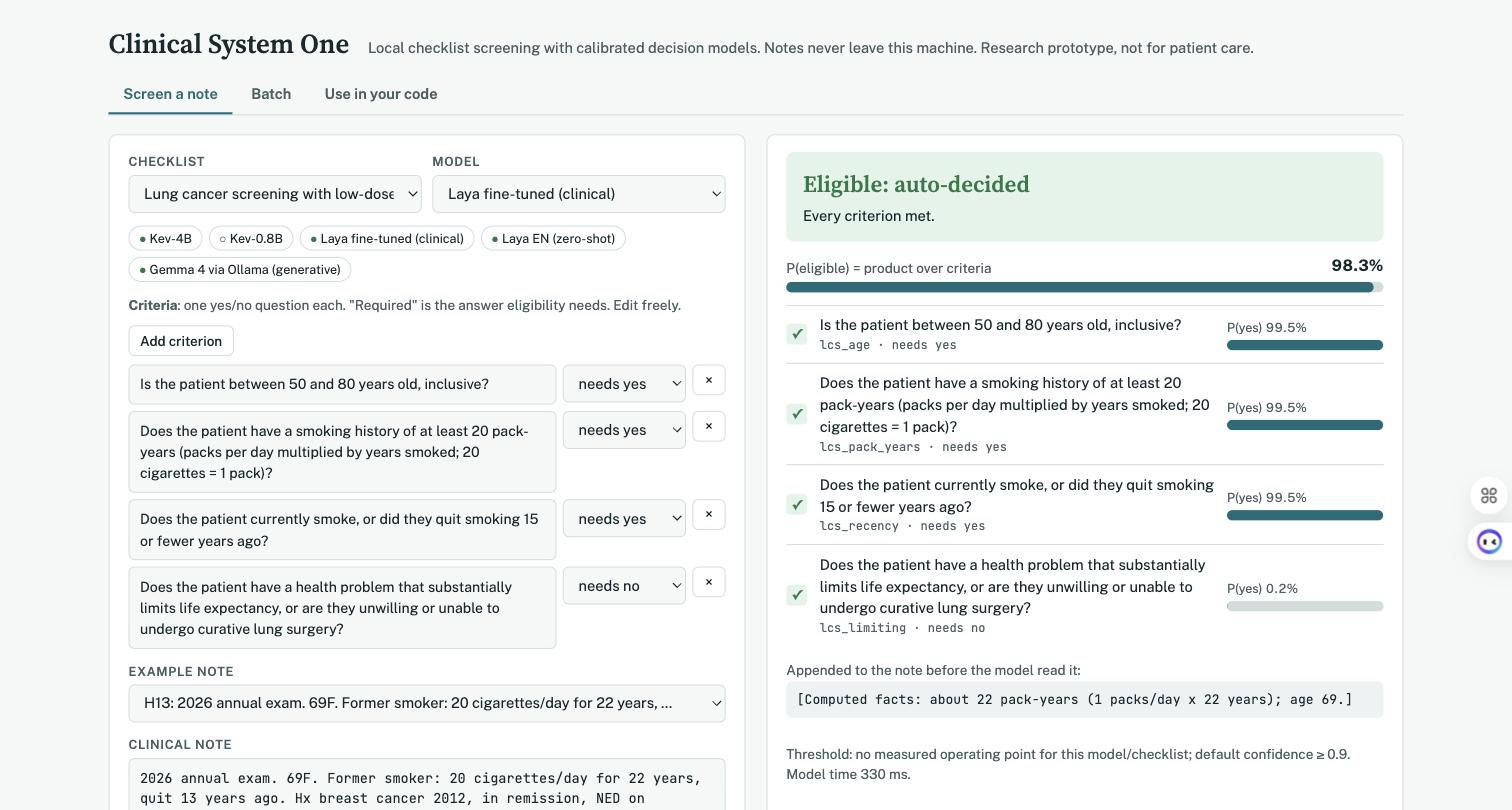
\includegraphics[width=\linewidth]{figures/app.png}
\caption{The released local screening app. Note, checklist and model are on the left; per-criterion $P(\text{yes})$, the conjunctive $P(\text{eligible})$, appended computed facts and the automation decision at the chosen error budget are on the right.}
\label{fig:app}
\end{figure}

\section{Question wording}
\label{app:questions}
\begin{small}
\paragraph{Lung cancer screening with low-dose CT (USPSTF 2021 (Grade B), JAMA 2021;325(10):962-970).}\begin{itemize}
\item \texttt{lcs\_age} (required: yes): Is the patient between 50 and 80 years old, inclusive?
\item \texttt{lcs\_pack\_years} (required: yes): Does the patient have a smoking history of at least 20 pack-years (packs per day multiplied by years smoked; 20 cigarettes = 1 pack)?
\item \texttt{lcs\_recency} (required: yes): Does the patient currently smoke, or did they quit smoking 15 or fewer years ago?
\item \texttt{lcs\_limiting} (required: no): Does the patient have a health problem that substantially limits life expectancy, or are they unwilling or unable to undergo curative lung surgery?
\item \texttt{lcs\_eligible} (direct): Under the USPSTF 2021 lung cancer screening recommendation (adults aged 50 to 80 years who have a 20 pack-year smoking history and currently smoke or have quit within the past 15 years, and who do not have a health problem that substantially limits life expectancy or the ability or willingness to have curative lung surgery), is this patient eligible for annual low-dose CT screening?\end{itemize}
\paragraph{One-time abdominal aortic aneurysm ultrasound screening (USPSTF 2019 (Grade B), JAMA 2019;322(22):2211-2218).}\begin{itemize}
\item \texttt{aaa\_male} (required: yes): Is the patient male?
\item \texttt{aaa\_age} (required: yes): Is the patient between 65 and 75 years old, inclusive?
\item \texttt{aaa\_ever\_smoked} (required: yes): Has the patient ever smoked tobacco (current or former smoker)?
\item \texttt{aaa\_eligible} (direct): Under the USPSTF 2019 recommendation (one-time ultrasound screening for abdominal aortic aneurysm in men aged 65 to 75 years who have ever smoked), is this patient eligible for AAA screening?\end{itemize}
\paragraph{TREC CT 2021.}\begin{itemize}
\item \texttt{eligible}: Based on the patient description, is this patient eligible for the clinical trial, meaning they satisfy the inclusion criteria and meet none of the exclusion criteria?
\item \texttt{meets\_inclusion}: Does the patient satisfy the trial's inclusion criteria?
\item \texttt{meets\_exclusion}: Does the patient meet any of the trial's exclusion criteria?
\end{itemize}
\end{small}

\section{Reproducing every number}
\begin{lstlisting}
experiments/prep_trec.py            # TREC CT 2021 sample + ClinicalTrials.gov criteria
experiments/run_all.sh              # original systems, one at a time, resumable
experiments/run_facts.sh            # computed-facts ablation
experiments/bench_model.sh          # any local System One server (new models)
experiments/analyze.py              # summary.json
experiments/figures.py; paper/make_tables.py
\end{lstlisting}
\end{document}
